\documentclass[../TDE4-E5.tex]{subfiles}%

\begin{document}
\section[s]"2"{Oscillateur amorti RLC à 2 mailles}

\enonce{%
	\noindent
	\begin{minipage}[c]{.65\linewidth}
		Considérons le circuit représenté ci-contre, où le condensateur est
		initialement déchargé. Le générateur fournit un échelon de tension, en passant
		de $0$ à $E$ à $t= 0$.
	\end{minipage}
	\hfill
	\begin{minipage}[c]{.32\linewidth}
		\begin{center}
			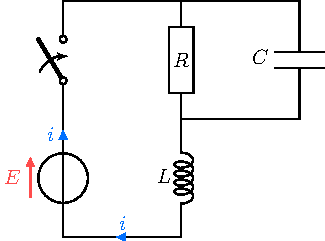
\includegraphics[width=\linewidth]{rlc_2mailles_plain}
		\end{center}
	\end{minipage}
}

\QR{%
	Établir l'équation différentielle vérifiée par le courant $i$.
}{
	\noindent
	\begin{minipage}[c]{.65\linewidth}
		On est en présence d'un circuit à deux mailles. On applique la loi des
		nœuds~:
		\begin{DispWithArrows*}
			i         & = i_R + i_C
			\Arrow{$i_C = C \dv{u}{t}$\\$i_R = \frac{u}{R}$}
			\\\Lra
			i         & = \frac{u}{R} + C \dv{u}{t}
			\intertext{Il faut changer $u$ en $i$. Or, $u_L = L \dv{i}{t}$~; il nous
				suffit donc de relier $u$ à $u_L$ par la loi des mailles~:}
			E         & = u + u_L
			\\\Lra
			u_L       & = E - u
		\end{DispWithArrows*}
	\end{minipage}
	\hfill
	\begin{minipage}[c]{.32\linewidth}
		\begin{center}
			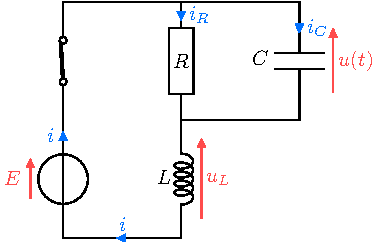
\includegraphics[width=\linewidth]{rlc_2mailles_flch}
		\end{center}
	\end{minipage}
	Ainsi, en réinjectant~:
	\begin{DispWithArrows*}
		i         & = \frac{E}{R} - \frac{u_L}{R} - C \dv{u_L}{t}
		\Arrow{$u_L = L \dv{i}{t}$}
		\\\Lra
		\Aboxed{i & = \frac{E}{R} - \frac{L}{R} \dv{i}{t} - LC \dv[2]{i}{t}}
	\end{DispWithArrows*}
}

\QR{%
L'écrire sous forme canonique en introduisant deux grandeurs $\omega_0$ et $Q$
que l'on interprétera.
}{%
On cherche à l'écrire sous la forme canonique classique
\[
	\frac{\dd^2 i}{\dd t^2} + \frac{\omega_0}{Q} \dv{i}{t} + {\omega_0}^2
	i = {\omega_0}^2 i_\infty
\]
L'identification à la forme précédente permet alors d'obtenir :
\[
	\omega_0 = \frac{1}{\sqrt{LC}}
	\qMath{,}
	Q = R\sqrt{\frac{C}{L}}
	\qet
	i_{\infty} = \frac{E}{R}
\]
Avec $\omega_0$ la pulsation propre de l'oscillateur, $Q$ le facteur de qualité
et $i_{\infty}$ la valeur prise par $i$ pour $t\to \infty$.
}

\QR{%
	Expliquer qualitativement l'expression du facteur de qualité.
}{%
	\textbf{Contrairement au RLC série}, $Q$ est proportionnel à $R$ (et non
	inversement proportionnel). C'est normal car ici, l'énergie est plus
	rapidement dissipée si $R$ est faible. Au contraire, si $R$ est élevée ($R\to
		\infty$), la branche contenant $R$ devient un interrupteur ouvert et le
	circuit devient équivalent à un oscillateur harmonique type LC série. $Q$ tend
	alors logiquement vers l'infini.
}%

\QR{%
	Donner la valeur du courant $i$ et de sa dérivée à l'instant initial.
}{%
	On étudie les conditions initiales grâce à deux schémas~:
	\smallbreak
	\noindent
	\begin{minipage}[c]{.45\linewidth}
		\vspace{0pt}
		\begin{center}
			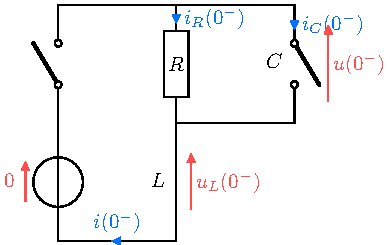
\includegraphics[width=\linewidth]{rlc_2mailles_0m}
			\captionof{figure}{Circuit à $\boxed{t = 0^-}$}
			\label{fig:t0m}
		\end{center}
	\end{minipage}
	\hfill
	\begin{minipage}[c]{.45\linewidth}
		\vspace{0pt}
		\begin{center}
			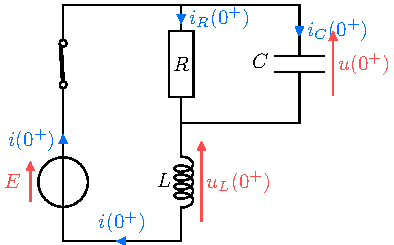
\includegraphics[width=\linewidth]{rlc_2mailles_0p}
			\captionof{figure}{Circuit à $\boxed{t = 0^+}$}
			\label{fig:t0p}
		\end{center}
	\end{minipage}
	\begin{itemize}
		\item Analysons le régime permanent à $t=0^-$, où le forçage est nul. Ce
		      régime est continu, donc la bobine y est équivalente à un fil. Ainsi,
		      d'après la loi des mailles,
		      \[
			      0 = u(0^-) + 0 \quad \text{donc} \quad u(0^-) = 0
		      \]
		      Par ailleurs, d'après la loi des nœuds,
		      \[
			      i(0^-) = i_R(0^-)+ i_C(0^-) = \frac{u(0^-)}{R}+0 = 0
		      \]
		      En effet, $i_C(0^-) = 0$ car le condensateur est équivalent à un
		      interrupteur ouvert en régime permanent.
		\item En $t=0^+$, la continuité de $i$ au travers de la bobine impose~:
		      \[
			      i(0^+) = i(0^-) = 0
		      \]
		      Afin de trouver la condition sur $\dv{i}{t}$, il faut déterminer la
		      valeur
		      de $u_L(0^+)$. Comme on cherche une tension, on utilise la loi des
		      mailles à $t=0^+$
		      \[
			      E = u(0^+)+ u_L(0^+)
		      \]
		      Or, $u$ étant la tension au borne d'un condensateur, elle est
		      nécessairement continue et égale à sa valeur en $0^-$ donc
		      \[
			      \boxed{u_L(0^+) = E
				      \qso
				      \dv{i}{t} (t=0^+) = \frac{E}{L}}
		      \]
	\end{itemize}
}

\QR{%
	En supposant $Q=2$, donner l'expression de $i(t)$ et tracer son allure.
}{%
	Le courant $i(t)$ s'écrit comme la somme d'une solution particulière de
	l'équation différentielle complète et d'une solution de l'équation homogène.
	Comme le forçage (qui se lit dans le second membre) est constant, le régime
	permanent (qui se lit dans la solution particulière) est constant aussi. La
	solution particulière est donc telle que
	\[
		0+0+\frac{1}{LC} i_p = \frac{E}{RLC} \quad \text{d'où} \quad i_p = \frac{E}{R}
	\]
	\underline{Remarque} : La solution $i_p$ déterminée sous forme d'une constante
	est toujours égale à $i_{\infty}$ identifiée dans la forme canonique.
	\medskip
	\smallbreak
	Pour trouver la solution homogène, écrivons l'équation caractéristique,
	\begin{gather*}
		r^2+ \frac{\omega_0}{Q} r + {\omega_0}^2 = 0
		\\\beforetext{$Q=2$ donc}
		\Delta = {\omega_0}^2 \pa{\frac{1}{4}-4} = -\frac{15}{4} {\omega_0}^2 <0
	\end{gather*}
	Les racines de l'équation caractéristique sont donc complexes conjuguées,
	\[
		r_{1,2} = -\frac{\omega_0}{4} \pm \jj \frac{\omega_0}{4} \sqrt{15}
		\qso
		r_{1,2} = -\mu \pm \jj \omega_p
	\]
	où $\mu$ est le taux d'amortissement et $\omega_p$ la pseudo-pulsation des
	oscillations. La solution homogène s'écrit alors
	\[
		i_h(t) = \text{e}^{-\mu t} \pa{A\cos(\omega_p t)+ B\sin(\omega_p t)}
	\]
	Avec $A$ et $B$ deux constantes d'intégration réelles. En sommant solution
	homogène et particulière, on obtient la solution générale :
	\[
		i(t) = \exr^{-\mu t} \pa{A\cos(\omega_p t)+ B\sin(\omega_p t)} + \frac{E}{R}
	\]
	Reste à déterminer les constantes d'intégration $A$ et $B$ en $t=0^+$
	\[
		i(0^+) = \frac{E}{R}+A = 0
		\qdc
		A = -\frac{E}{R}
	\]
	Calculons l'expression de la dérivée
	\begin{gather*}
		\dv{i}{t} = \omega_p \pac{-A\sin(\omega_p t)+ B \cos(\omega_p t)}
		\exr^{-\mu t} - \mu \pac{A\cos(\omega_p t)+ B \sin(\omega_p t)}
		\exr^{-\mu t}
		\\
		\beforetext{Ainsi}
		\qty(\dv{i}{t})_{0^+} =
		B\omega_p - \mu A = \frac{E}{L}
		\qdc
		B = \frac{E}{\omega_p} \pa{\frac{1}{L} - \frac{\mu}{R}}
		\\\beforetext{Finalement}
		i(t) =
		\frac{E}{R} -
		\frac{E}{R}\exr^{-\mu t}
		\pac{%
			\cos(\omega_p t) -
			\frac{R}{\omega_p}
			\pa{%
				\frac{1}{L} - \frac{\mu}{R}
			}%
			\sin(\omega_p t)
		}
	\end{gather*}

	\noindent
	\begin{minipage}[c]{.48\linewidth}
		Le tracé «~direct~» n'est pas possible, il faut donc utiliser les
		informations à disposition : conditions initiales, qui donne la valeur à $t
			= 0$ et le signe de la pente de la tangente, régime pseudo-périodique avec
		environ $Q = 2$ oscillations, et solution particulière qui donne le régime
		permanent asymptotique. Un exemple de chronogramme acceptable est représenté
		figure ci-contre).
	\end{minipage}
	\begin{minipage}[c]{.48\linewidth}
		\begin{center}
			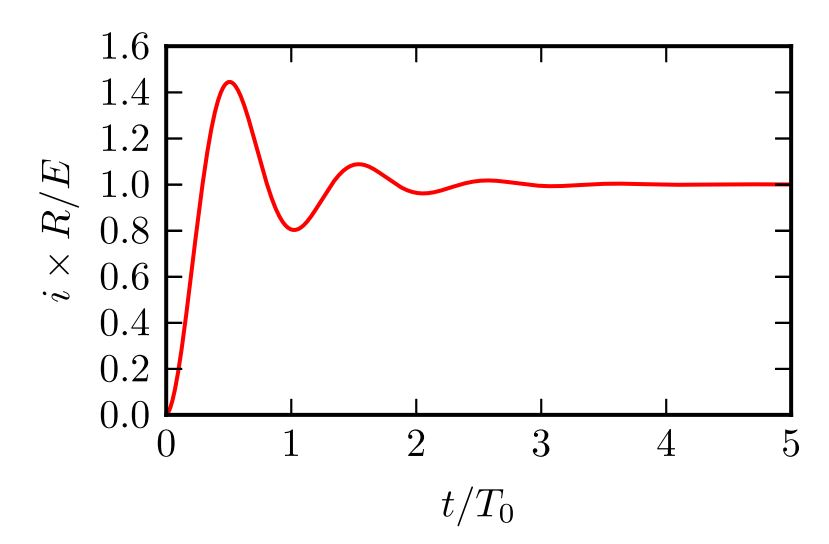
\includegraphics[width=\linewidth]{corrige2}
		\end{center}
	\end{minipage}
}%

\end{document}
